\section{Evaluation}
\label{sec:evaluation}

To quantify and better understand the VM delivery approaches discussed
in Section~\ref{sec:vmdelivery}, we have conducted a number of
experiments on our prototype.  Since bulk transfer is straightforward,
we focus on demand paging and synthesis. We ask two questions in each experiment:
\begin{smitemize} 
\item{What is the total time and breakdown to
deliver a VM, launch it, and perform an offload operation?}

\item{How does energy consumption on the mobile device differ across approaches?}
\end{smitemize}

\subsection{Applications \& Experimental Setup}
\label{sec:setup}

We offloaded four applications on a cloudlet:
\paragraph{OBJECT:}~Linux C++ application based
on the CMU MOPED object recognition libraries~\cite{MOPED2011}. 
It returns the identities of recognized objects in an input image.

\paragraph{FACE:}~Windows XP C++ application
based on the OpenCV library~\cite{OPENCV2011}. It
returns the coordinates and identities of recognized faces in an input image.

\paragraph{SPEECH:}~Windows XP Java application
based on the CMU Sphinx-4 speech recognition
toolkit~\cite{Sphinx2011}. It returns a text transcription of a WAV input
file.

\paragraph{NULL:}~Empty application to serve as a baseline.


\begin{figure}
\centering
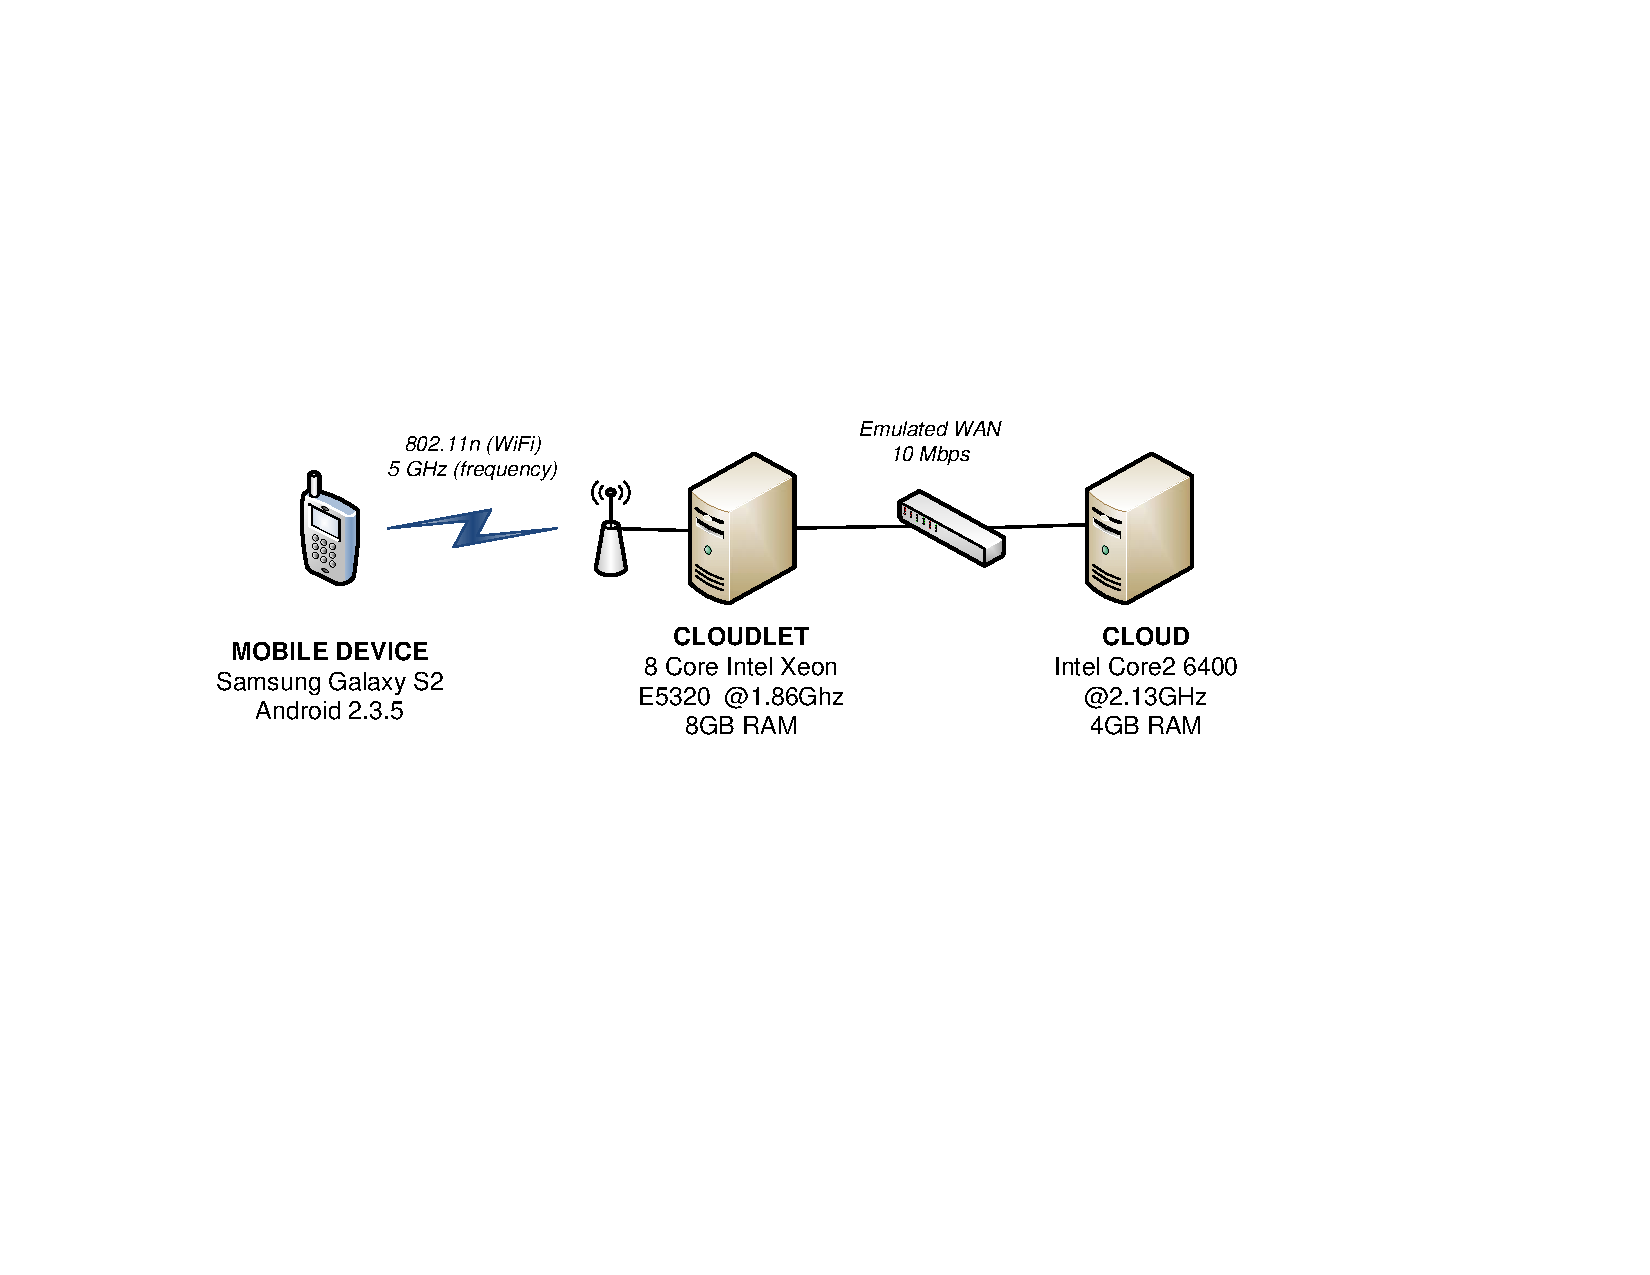
\psfig{file=FIGS/fig-experiment-setup.pdf, scale=0.4}
\vspace{-0.1in}
\caption{Experimental Setup}
\vspace{-0.2in}
\label{fig:exp-setup}
\end{figure}

All experiments were conducted using the configuration shown in
Figure~\ref{fig:exp-setup}.  The mobile device is a Samsung Galaxy S2
smartphone running Android 2.3.5. It connects to the cloudlet via
802.11n Wi-Fi at 5 GHz.  The cloudlet is connected to the cloud via a
1~Gbps Ethernet and a network emulator that can throttle bandwidth to
emulate a WAN.  We measured energy usage with a Power Monitor from
Monsoon Solutions Inc. and the corresponding Power Tool
software~\cite{Monsoon2011}.  To ensure good experimental control, we
scripted all interactive inputs.  Three runs of each experiment were
done.  Since observed standard deviations were low (less than
$4\%$ for time and less than $5\%$ for energy) they are not
explicitly shown in our results.

\subsection{Benchmarks and Metrics} 
\label{sec:benchmarks}

We established four benchmarks that map to the demand paging and synthesis
strategies presented in Section~\ref{sec:vmdelivery}. In each of these 
cases the VM launch is initiated by the mobile device.

\paragraph{Demand Page from Cloud~$(D_{cloud})$:}~The cloudlet 
retrieves the VM memory snapshot and VM disk image metadata from the cloud and 
launches the VM using only the memory snapshot. The VM disk 
image remains on the cloud and pages are retrieved on demand. 

\paragraph{Demand Page from Mobile~$(D_{mobile})$:}~Similar to the previous
benchmark with the difference that the VM memory snapshot and VM disk 
image metadata are retrieved from the mobile device and the VM disk image
remains on the mobile device. 

\paragraph{Synthesis from Cloud~$(S_{cloud})$:}~The cloudlet contains the 
base VM disk image and the base VM memory snapshot. It retrieves the VM 
disk overlay and the VM memory snapshot overlay from the cloud and applies 
them to the base disk image and base memory snapshot. After that, the
cloudlet launches the VM.

\paragraph{Synthesis from Mobile~$(S_{mobile})$:}~Similar to the previous
benchmark with the difference that the VM disk image overlay and VM memory 
snapshot overlay are retrieved from the mobile device instead of the cloud.

\begin{table}
\centering
\begin{small}
\begin{tabular} {rcccc}
\hline\hline
&&&VM Disk&Compr\\
&App&VM Disk&Image&VM Mem\\
&Size&Image&Metadata&Snapshot\\
App&(MB)&(GB)&(MB)&(MB)\\ 
\hline
OBJECT&27.50&2.48&5.45&136\\
FACE&17.65&1.57&5.45&121\\
SPEECH&51.04&1.57&5.45&189\\
NULL&0.00&2.48&5.45&65\\
\hline
\end{tabular}
\end{small}
\caption{VM Information for Demand Paging}
\label{table:demandpagesizes}
\end{table}


\begin{table}
\centering
\begin{small}
\begin{tabular} {rcccccc}
\hline\hline
&&&&Compr&Compr\\
&&Base&Base&Disk&Mem\\
&App&Disk&Mem&Image&Snap\\
&Size&Image&Snap&Ovlay&Ovlay\\
App&(MB)&(GB)&(MB)&(MB)&(MB)\\
\hline
OBJECT&27.5&2.50&474.49&30.27&134.55 \\
FACE&17.65&1.61&357.69&50.54&44.13 \\
SPEECH&51.04&1.61&357.69&96.60&89.23 \\
NULL&0.00&2.50&474.49&0.01&0.12\\
\hline
\end{tabular}
\end{small}
\vspace{-0.1in}
\caption{VM Information for Synthesis Cases}
\label{table:synthesissizes}
\vspace{-0.2in}
\end {table}

Table~\ref{table:demandpagesizes} and Table~\ref{table:synthesissizes}
show VM information for the demand paging and synthesis cases.  The
metrics captured during the experiments were end-to-end VM launch
time, first run time, and energy consumption on the mobile device.  In
the demand paging cases, VM launch time is the sum of memory snapshot
transfer time, disk image metadata transfer time, snapshot
decompression time and VM resume time. In the synthesis cases VM
launch time is the sum of VM disk image overlay transfer time, VM
memory snapshot overlay transfer time, overlay decompression time, VM
synthesis time and VM resume time.


\subsection{Results and Discussion}
\label{sec:results}

\begin{figure*}
\centering
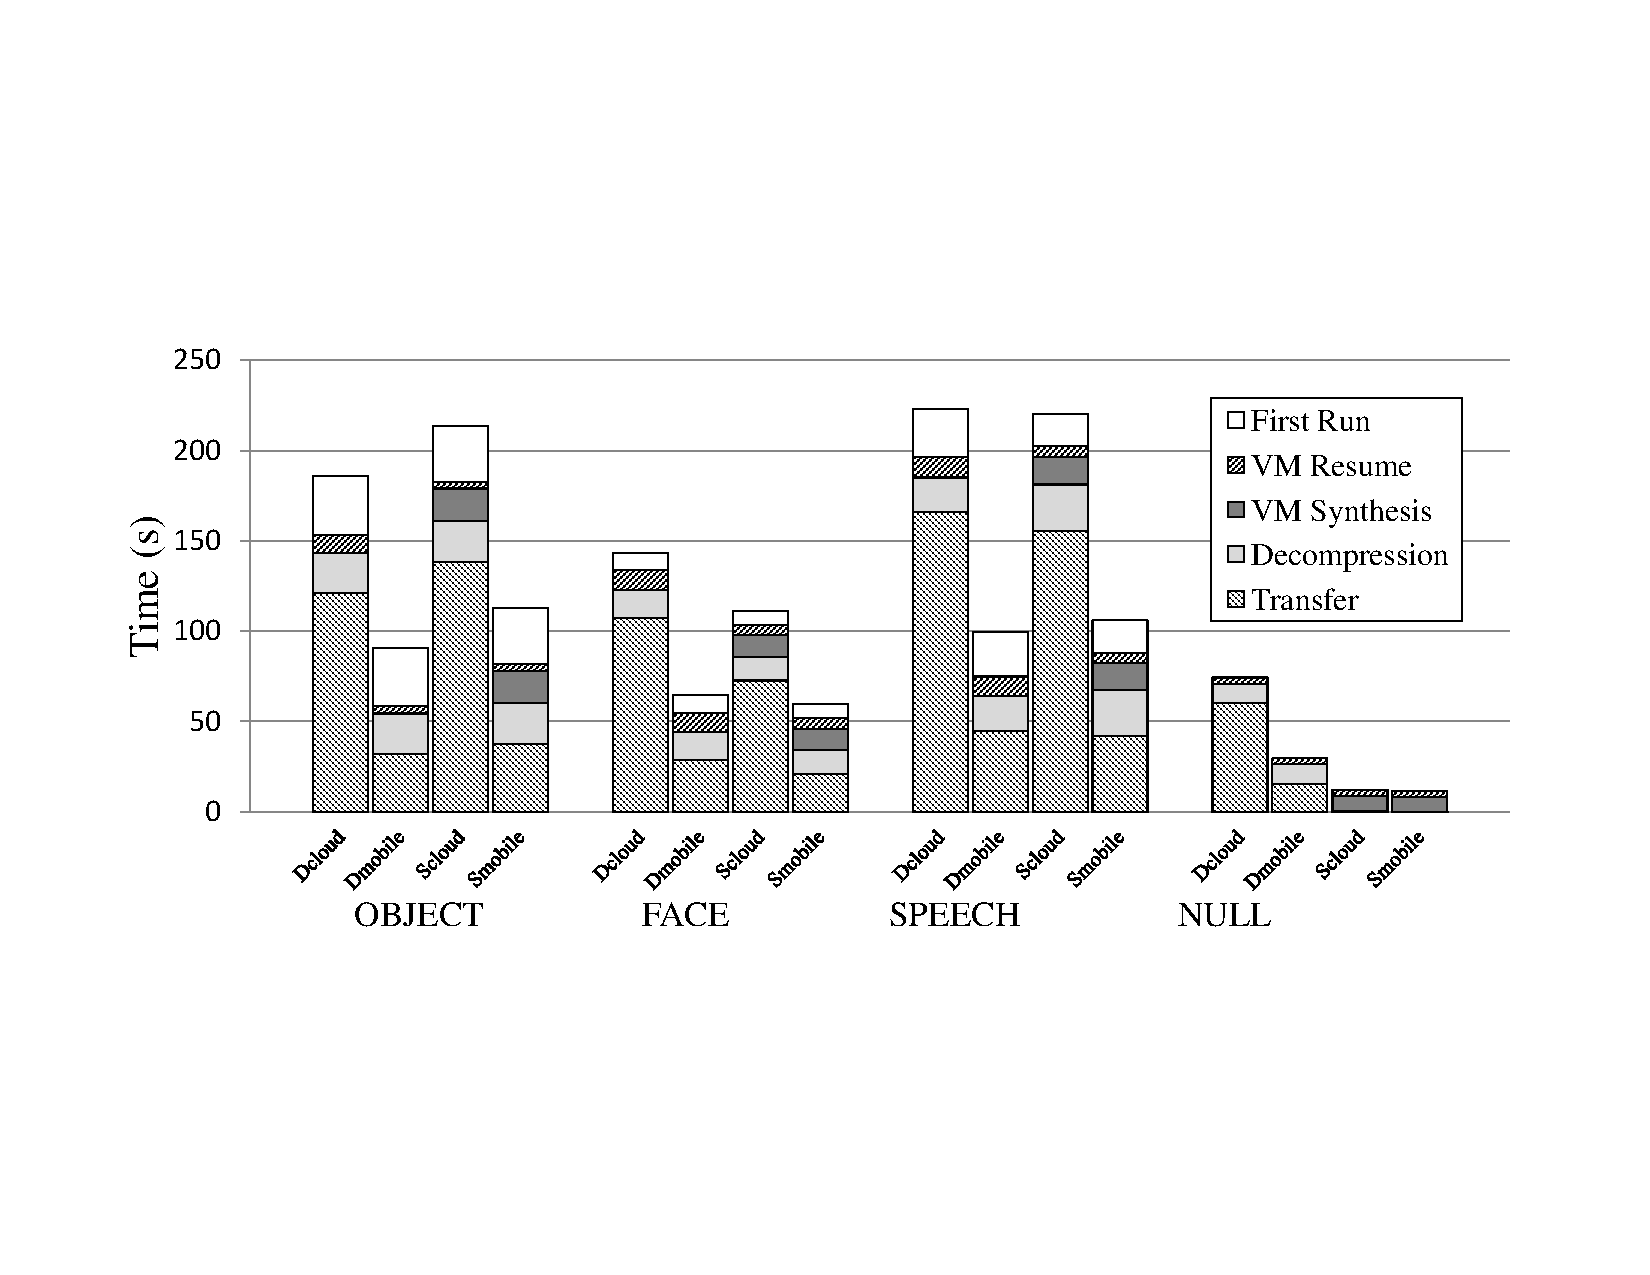
\psfig{file=FIGS/fig-benchmark-app.pdf, scale=0.5}
\vspace{-0.2in}
\caption{Total Benchmark Time}
\vspace{-0.2in}
\label{fig:benchmark-time}
\end{figure*}

\paragraph{End-to-End VM Launch Time:}~Figure~\ref{fig:benchmark-time}
shows benchmark results for the different VM delivery strategies for
each application. The graph shows that data transfer is the largest
component of end-to-end VM launch time and that it is greater for the
VM delivery strategies from the cloud. This is expected because the
bandwidth is smaller for cloud-cloudlet communication (10 Mbps).  The mobile
device used in our experiments supports 32--38 Mbps. Data transfer
times should be even smaller with other shorter-range,
higher-bandwidth networks.

The graph also shows the effect of VM image size. The synthesis strategies
transfer only the overlays for the VM image which contain the parts that
are specific to the application being offloaded. As shown in Tables 
~\ref{table:demandpagesizes} and ~\ref{table:synthesissizes} the overlays 
for the most part are much smaller in size compared to the full VM image
size. For the FACE application, for example,  the disk overlay is $3.2\%$ 
of the disk image and the memory overlay is $36\%$ of the memory snapshot. 
Because overlays are smaller, end-to-end VM launch time for synthesis is 
expected to be smaller than for demand paging even if both the VM image and 
memory snapshot overlays have to be transferred before the VM can be 
launched. However, if the application requires a lot of disk space or 
memory then the sum of the sizes of the two overlays could be greater than 
the size of the memory snapshot required for demand paging. This is the 
case with OBJECT, where the disk overlay is $1.2\%$ of the 
disk image but the memory overlay is $98\%$ of the memory snapshot, which 
explains the greater end-to-end VM launch times for the synthesis 
strategies.

\begin{figure}
\centering
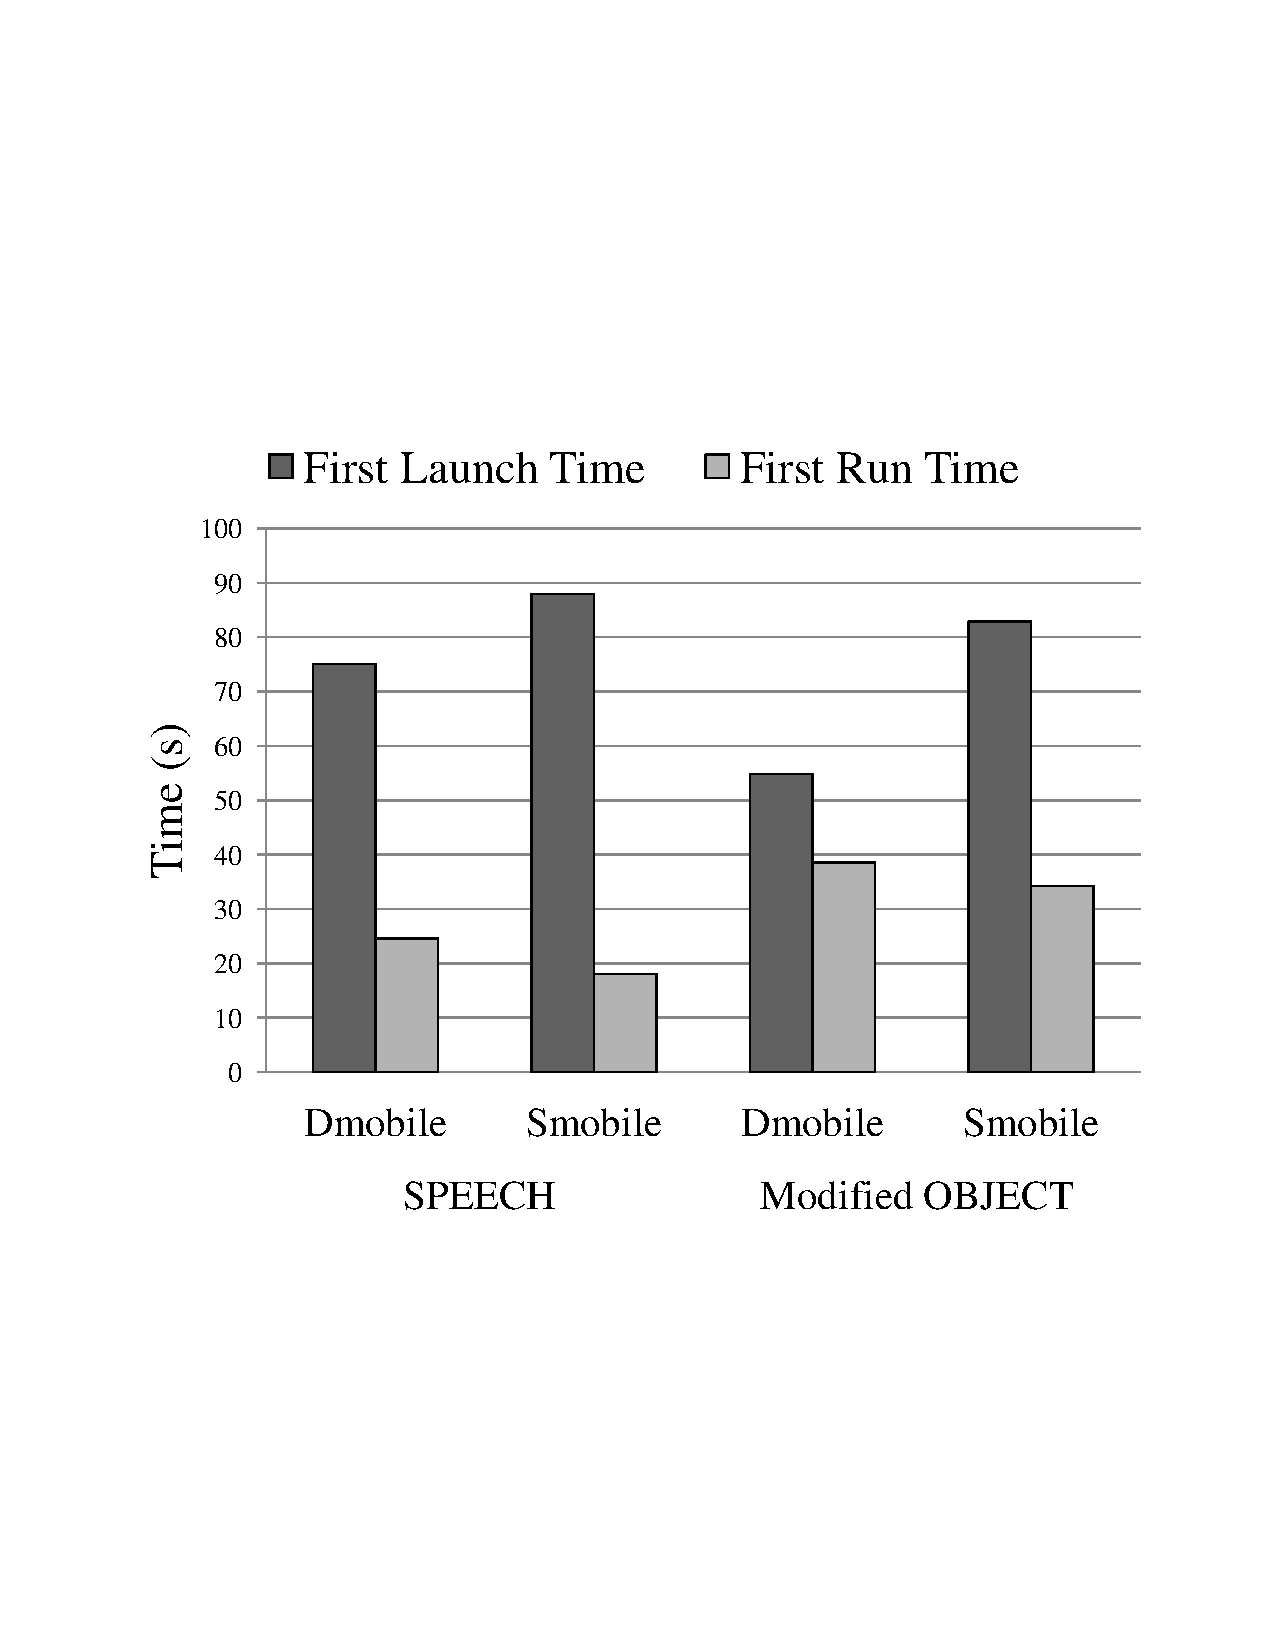
\psfig{file=FIGS/fig-benchmark-demand-synthesis.pdf, scale=0.35}
\vspace{-0.2in}
\caption{Demand Paging vs. Synthesis}
\vspace{-0.2in}
\label{fig:demand_synthesis}
\end{figure}

\paragraph{Application Execution Time:}~
Figure~\ref{fig:benchmark-time} shows that first run time is
very similar between the demand paging and synthesis strategies for all
applications. The only one that shows a slight difference is SPEECH
(demand paging takes 9 more seconds than synthesis). This is contrary to
our intuition because we expected demand paging to have
greater first run times. The rationale is that although demand paging
can generate the launch VM faster because it only requires the VM memory snapshot,
it requires disk page fetching during the first
run because it has no disk image data. SPEECH is the most data-intensive
application because it reads large language model files.
This explains why it shows a slight difference in first run times.


To further understand the effects of demand paging on data-intensive 
applications we modified OBJECT so that it would load
the object-modeling files (25MB) upon client request instead of having 
them pre-loaded in memory, which would make them part of the VM memory 
snapshot. Figure~\ref{fig:demand_synthesis} shows the original SPEECH
data along with the results of modified OBJECT.
In both cases, we can clearly see that the synthesis strategy has a smaller
first run time but a larger first launch time which is consistent with our
intuition. This difference does not appear to be significant because 
data transfer time is still the dominant part of end-to-end VM launch time.
However, the effect of demand paging will increase linearly as the size of 
the files increases over time due to additional training or object-modeling
files. 

\begin{figure}
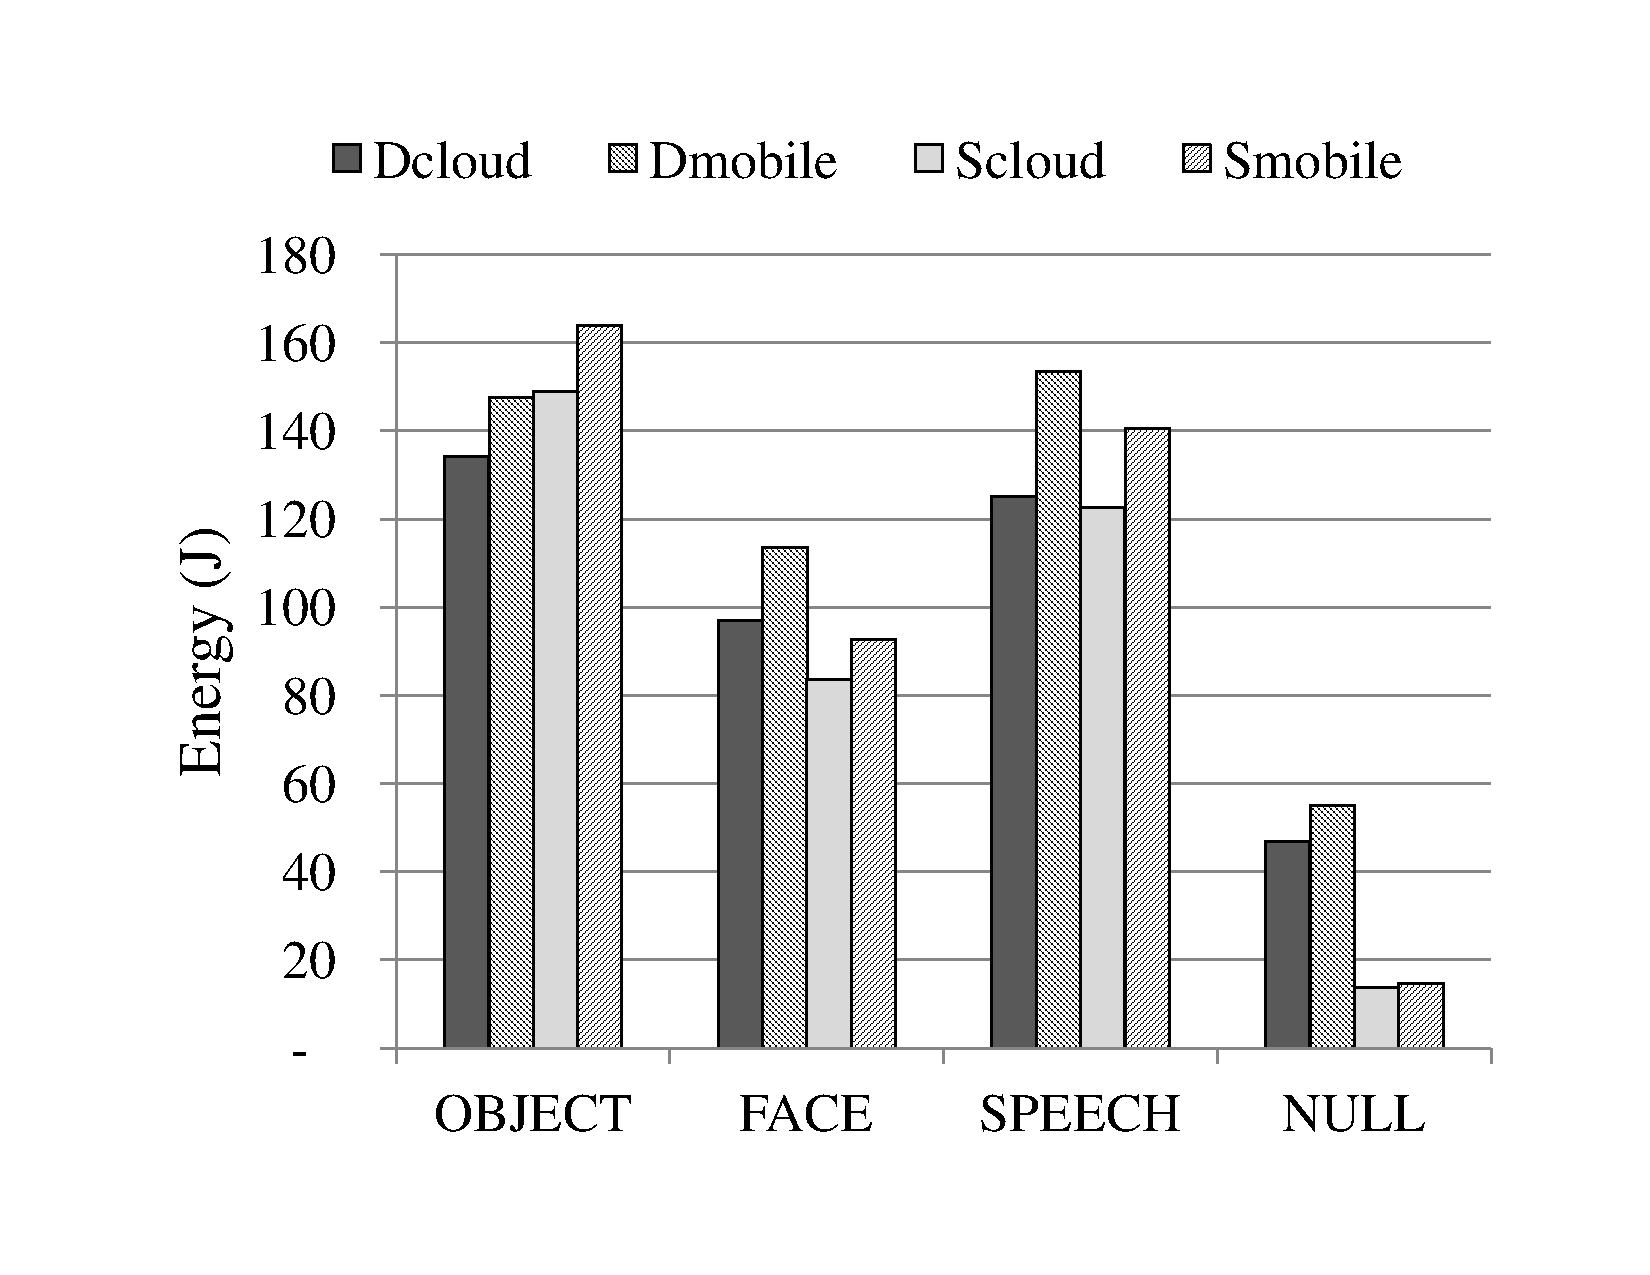
\psfig{file=FIGS/fig-benchmark-energy.pdf, scale=0.3}
\vspace{-0.2in}
\caption{Energy consumption on mobile device}
\vspace{-0.2in}
\label{fig:benchmark-energy}
\end{figure}


\paragraph{Energy :}~
Energy consumption in all the experiments is measured from the moment
that the mobile device initiates VM launch until the first run ends.
Figure~\ref{fig:benchmark-energy} shows that $D_{mobile}$ and
$S_{mobile}$ consume more energy than $D_{cloud}$ and $S_{cloud}$
respectively. The average energy savings is $14.3\%$ for demand paging
cases and $9.6\%$ for synthesis cases. These savings seem
small. However, data transfer from the cloud takes approximately twice
as long as from the mobile device (see
Figure~\ref{fig:benchmark-time}) and during this time the mobile
device is in the idle state waiting for a response.  Our experiments
show that average power in the idle state is 430.44 mW, which is
significant and contributes to this lower than expected savings.

